%% BioMed_Central_Tex_Template_v1.06
%%                                      %
%  bmc_article.tex            ver: 1.06 %
%                                       %

%%IMPORTANT: do not delete the first line of this template
%%It must be present to enable the BMC Submission system to
%%recognise this template!!

%%%%%%%%%%%%%%%%%%%%%%%%%%%%%%%%%%%%%%%%%
%%                                     %%
%%  LaTeX template for BioMed Central  %%
%%     journal article submissions     %%
%%                                     %%
%%          <8 June 2012>              %%
%%                                     %%
%%                                     %%
%%%%%%%%%%%%%%%%%%%%%%%%%%%%%%%%%%%%%%%%%


%%%%%%%%%%%%%%%%%%%%%%%%%%%%%%%%%%%%%%%%%%%%%%%%%%%%%%%%%%%%%%%%%%%%%
%%                                                                 %%
%% For instructions on how to fill out this Tex template           %%
%% document please refer to Readme.html and the instructions for   %%
%% authors page on the biomed central website                      %%
%% http://www.biomedcentral.com/info/authors/                      %%
%%                                                                 %%
%% Please do not use \input{...} to include other tex files.       %%
%% Submit your LaTeX manuscript as one .tex document.              %%
%%                                                                 %%
%% All additional figures and files should be attached             %%
%% separately and not embedded in the \TeX\ document itself.       %%
%%                                                                 %%
%% BioMed Central currently use the MikTex distribution of         %%
%% TeX for Windows) of TeX and LaTeX.  This is available from      %%
%% http://www.miktex.org                                           %%
%%                                                                 %%
%%%%%%%%%%%%%%%%%%%%%%%%%%%%%%%%%%%%%%%%%%%%%%%%%%%%%%%%%%%%%%%%%%%%%

%%% additional documentclass options:
%  [doublespacing]
%  [linenumbers]   - put the line numbers on margins

%%% loading packages, author definitions

%\documentclass[twocolumn]{bmcart}% uncomment this for twocolumn layout and comment line below
\documentclass{bmcart}

%%% Load packages
%\usepackage{amsthm,amsmath}
%\RequirePackage{natbib}
\RequirePackage{natbib}% uncomment this for author-year bibliography
%\RequirePackage{hyperref}
\usepackage[utf8]{inputenc} %unicode support
%\usepackage[applemac]{inputenc} %applemac support if unicode package fails
%\usepackage[latin1]{inputenc} %UNIX support if unicode package fails

%%%%%%%%%%%%%%%%%%%%%%%%%%%%%%%%%%%%%%%%%%%%%%%%%
%%                                             %%
%%  If you wish to display your graphics for   %%
%%  your own use using includegraphic or       %%
%%  includegraphics, then comment out the      %%
%%  following two lines of code.               %%
%%  NB: These line *must* be included when     %%
%%  submitting to BMC.                         %%
%%  All figure files must be submitted as      %%
%%  separate graphics through the BMC          %%
%%  submission process, not included in the    %%
%%  submitted article.                         %%
%%                                             %%
%%%%%%%%%%%%%%%%%%%%%%%%%%%%%%%%%%%%%%%%%%%%%%%%%

\usepackage{todonotes}
\usepackage{graphicx}
\usepackage{amsmath}
\usepackage{url}
\usepackage{subcaption}
\usepackage{booktabs}
%\def\includegraphic{}
%\def\includegraphics{}



%%% Put your definitions there:
\startlocaldefs
\endlocaldefs


%%% Begin ...
\begin{document}
	
	%%% Start of article front matter
	\begin{frontmatter}
		
		\begin{fmbox}
			\dochead{Methodology}
			
			%%%%%%%%%%%%%%%%%%%%%%%%%%%%%%%%%%%%%%%%%%%%%%
			%%                                          %%
			%% Enter the title of your article here     %%
			%%                                          %%
			%%%%%%%%%%%%%%%%%%%%%%%%%%%%%%%%%%%%%%%%%%%%%%
			
			\title{Statistical Stopping Criteria for Active Learning in Systematic Review Screening}
			
			%%%%%%%%%%%%%%%%%%%%%%%%%%%%%%%%%%%%%%%%%%%%%%
			%%                                          %%
			%% Enter the authors here                   %%
			%%                                          %%
			%% Specify information, if available,       %%
			%% in the form:                             %%
			%%   <key>={<id1>,<id2>}                    %%
			%%   <key>=                                 %%
			%% Comment or delete the keys which are     %%
			%% not used. Repeat \author command as much %%
			%% as required.                             %%
			%%                                          %%
			%%%%%%%%%%%%%%%%%%%%%%%%%%%%%%%%%%%%%%%%%%%%%%
			
			\author[
			addressref={aff1,aff2},                   % id's of addresses, e.g. {aff1,aff2}
			corref={aff1},                       % id of corresponding address, if any
			%noteref={n1},                        % id's of article notes, if any
			email={callaghan@mcc-berlin.net}   % email address
			]{\inits{MW}\fnm{Max W} \snm{Callaghan}}
			\author[
			addressref={aff1, aff3},
			email={mueller-hansen@mcc-berlin.net}
			]{\inits{FMH}\fnm{Finn} \snm{M\"{u}ller-Hansen}}
			
			%%%%%%%%%%%%%%%%%%%%%%%%%%%%%%%%%%%%%%%%%%%%%%
			%%                                          %%
			%% Enter the authors' addresses here        %%
			%%                                          %%
			%% Repeat \address commands as much as      %%
			%% required.                                %%
			%%                                          %%
			%%%%%%%%%%%%%%%%%%%%%%%%%%%%%%%%%%%%%%%%%%%%%%
			
			\address[id=aff1]{%                           % unique id
				\orgname{Mercator Research Institute on Global Commons and Climate Change}, % university, etc
				\street{Torgauer Straße},                     %
				\postcode{10829}                                % post or zip code
				\city{Berlin},                              % city
				\cny{Germany}                                    % country
			}
			\address[id=aff2]{%
				\orgname{Priestley International Centre for Climate, University of Leeds, Leeds },
				%\street{Dsternbrooker Weg 20},
				\postcode{LS2 9JT}
				\city{Leeds},
				\cny{United Kingdom}
			}
			\address[id=aff3]{%
				\orgname{Potsdam Institute for Climate Impact Research (PIK), Member of the Leibniz Association},
				\street{P.O. Box 60 12 03},
				\postcode{D-14412}
				\city{Potsdam},
				\cny{Germany}
			}
			
			%%%%%%%%%%%%%%%%%%%%%%%%%%%%%%%%%%%%%%%%%%%%%%
			%%                                          %%
			%% Enter short notes here                   %%
			%%                                          %%
			%% Short notes will be after addresses      %%
			%% on first page.                           %%
			%%                                          %%
			%%%%%%%%%%%%%%%%%%%%%%%%%%%%%%%%%%%%%%%%%%%%%%
			
			\begin{artnotes}
				%\note{Sample of title note}     % note to the article
				%\note[id=n1]{Equal contributor} % note, connected to author
			\end{artnotes}
			
		\end{fmbox}% comment this for two column layout
		
		%%%%%%%%%%%%%%%%%%%%%%%%%%%%%%%%%%%%%%%%%%%%%%
		%%                                          %%
		%% The Abstract begins here                 %%
		%%                                          %%
		%% Please refer to the Instructions for     %%
		%% authors on http://www.biomedcentral.com  %%
		%% and include the section headings         %%
		%% accordingly for your article type.       %%
		%%                                          %%
		%%%%%%%%%%%%%%%%%%%%%%%%%%%%%%%%%%%%%%%%%%%%%%
		
		\begin{abstractbox}
			
			\begin{abstract} % abstract
				%\parttitle{First part title} %if any
				Active learning for systematic review screening promises to reduce the human effort required to identify relevant documents for a systematic review. 
				Machines and humans  work together, with humans providing training data, and the machine optimising the documents that the humans screen. This enables the identification of all relevant documents after viewing only a fraction of the total documents. 
				However, current approaches lack robust stopping criteria, so that reviewers do not know when they have seen all or a certain proportion of relevant documents. This means that such systems are hard to implement in live reviews. 
				This paper introduces a workflow with robust and flexible statistical stopping criteria, which offer real work reductions on the basis of a given confidence level of reaching a given recall.
				The stopping criteria are shown on test datasets to achieve a reliable level of recall, while still providing consistent work reductions, while other methods proposed are shown to provide inconsistent recall and work reductions across datasets.
				
			\end{abstract}
			
			%%%%%%%%%%%%%%%%%%%%%%%%%%%%%%%%%%%%%%%%%%%%%%
			%%                                          %%
			%% The keywords begin here                  %%
			%%                                          %%
			%% Put each keyword in separate \kwd{}.     %%
			%%                                          %%
			%%%%%%%%%%%%%%%%%%%%%%%%%%%%%%%%%%%%%%%%%%%%%%
			
			\begin{keyword}
				\kwd{Systematic Review}
				\kwd{Machine Learning}
				\kwd{Active Learning}
				\kwd{Stopping Criteria}
			\end{keyword}
			
			% MSC classifications codes, if any
			%\begin{keyword}[class=AMS]
			%\kwd[Primary ]{}
			%\kwd{}
			%\kwd[; secondary ]{}
			%\end{keyword}
			
		\end{abstractbox}
		%
		%\end{fmbox}% uncomment this for twcolumn layout
		
	\end{frontmatter}

%%%%%%%%%%%%%%%%%%%%%%%%%%%%%%%%%%%%%%%%%%%%%%
%%                                          %%
%% The Main Body begins here                %%
%%                                          %%
%% Please refer to the instructions for     %%
%% authors on:                              %%
%% http://www.biomedcentral.com/info/authors%%
%% and include the section headings         %%
%% accordingly for your article type.       %%
%%                                          %%
%% See the Results and Discussion section   %%
%% for details on how to create sub-sections%%
%%                                          %%
%% use \cite{...} to cite references        %%
%%  \cite{koon} and                         %%
%%  \cite{oreg,khar,zvai,xjon,schn,pond}    %%
%%  \nocite{smith,marg,hunn,advi,koha,mouse}%%
%%                                          %%
%%%%%%%%%%%%%%%%%%%%%%%%%%%%%%%%%%%%%%%%%%%%%%

%%%%%%%%%%%%%%%%%%%%%%%%% start of article main body
% <put your article body there>

%%%%%%%%%%%%%%%%
%% Background %%
%%
	
	%%%%%%%%%%%%%%%%%%%%%%%%
	%% Introduction
	\section*{Background}
	
	Evidence synthesis technology is a rapidly emerging field that promises to change the practice of evidence synthesis work \cite{Westgate2018}.
	Interventions have been proposed at various points in order to reduce the human effort required to produce systematic reviews and other forms of evidence synthesis.
	A major strand of the literature works on screening: the identification of relevant documents in a set of documents whose relevance is uncertain \cite{OMara-Eves2015}. 
	This is a time consuming and repetitive task, and in a research environment with constrained resources and increasing amounts of literature, this may limit the scope of the evidence synthesis projects undertaken.
	Several papers have developed Active Learning (AL) approaches \cite{miwa2014, Wallace2010a, Wallace2010, Jonnalagadda2013, Przybya2018} to reduce the time required to screen documents. This paper sets out how current approaches are  unsuitable in practice, and outlines and evaluates a small modification that would make AL systems ready for live reviews.
	
	Active learning is an iterative process where documents screened by humans are used to train a machine learning model to predict the relevance of unseen papers \cite{Settles2009}.
	The algorithm chooses which studies will next be screened by humans, often those which are likely to be relevant or about which the model is uncertain, in order to generate more labels to feed back to the machine. 
	By prioritising those studies most likely to be relevant, a human reviewer most often identifies all relevant studies - or a given proportion of relevant studies (recall) - before having seen all the documents in the corpus. 
	The proportion of documents not yet seen by the human when they reach the given recall threshold is referred to as the work saved. This represents the proportion of documents that they do not have to screen, which they would have had to without machine learning.
	
	Machine learning applications are often evaluated using sets of documents from already completed systematic reviews for which inclusion or exclusion labels already exist. 
	As all human labels are known \textit{a priori}, it is possible to simulate the screening process, recording when a given recall target has been achieved.
	In live review settings, however, recall remains unknown until all documents have been screened. 
	In order for work to really be saved, reviewers have to stop screening while uncertain about recall. 
	This is particularly problematic in systematic reviews because low recall increases the risk of bias \cite{Lefebvre2011}.
	The lack of appropriate stopping criteria has therefore been identified as a research gap \cite{bannach-brown2019}, although some approaches have been suggested. These fall into the following categories:
	\begin{itemize}
		\item \textbf{Sampling criteria:} Reviewers estimate the number of relevant documents by taking a random sample at the start of the process. They stop when this number, or a given proportion of it, has been reached \cite{Shemilt2014}
		\item \textbf{Heuristics:} Reviewers stop when a given number of irrelevant articles are seen in a row \cite{Jonnalagadda2013, Przybya2018}. 
		\item \textbf{Pragmatic criteria:} Reviewers stop when they run out of time \cite{miwa2014}. 
	\end{itemize}
	
	We show in this paper how existing criteria are inadequate.
	We demonstrate with several previously used datasets that their inadequacy lies in the unreliability - particularly across different domains, or datasets with different properties \cite{OMara-Eves2015} - both of the work saved and the recall achieved.  
	Without the reliable or reportable achievement of a desired level of recall, deployment of AL systems in live reviews remains challenging.
	
	This study proposes a system for estimating the recall based on random sampling of remaining documents. 
	We use a simple statistical method to iteratively test a null hypothesis that the recall achieved is less than a given target recall. If the hypothesis can be rejected, we conclude that the recall target has been achieved with a given confidence level and screening can be stopped.
	This allows AL users to predefine a target in terms of uncertainty and recall, so that they can make transparent, easily communicable statements like ``There is a <5\% chance that we achieve a recall under 95\%''.
	
	The information retrieval literature discusses similar stopping criteria for ranking algorithms like BM25 and variants \cite{DiNunzio2018, Yu2019}. However, the estimators they use to determine the recall rely on the specific ranking functions and depend on their search input. Therefore, the quality of the estimation depends on the adequacy of the model. Our approach, on the contrary, is independent of model choice or model performance. 
	
	In the remainder of the paper, we first discuss in detail the shortcomings of existing stopping criteria. Then, we introduce our new criterion based on a hypergeometric test. We evaluate our stopping criteria, and compare their performance with heuristic and sampling based criteria on real-world systematic review datasets on which AL systems have previously been tested \cite{Cohen2006, Yu2019, Terasawa2009, Castaldi2009}.
	
	\section*{Methods}

	
	%\subsection*{Existing Stopping Criteria for Active Learning}
	
	We start by explaining the sampling and heuristic based stopping criteria and showing their methodological weaknesses. 
	
	\subsection*{Sampling Based Stopping Criteria}
	
	The stopping criterion suggested by Shemilt et al. \cite{Shemilt2014} involves establishing the Baseline Inclusion Rate (BIR), by taking a random sample at the beginning of screening. 
	The BIR is used to estimate the number of relevant documents in the whole dataset. 
	Reviewers continue to screen until this number, or a proportion of it corresponding to the desired level of recall, is reached.
	

	
	However, the estimation of the BIR fails to correctly take into account sampling uncertainty \footnote{Although Shemilt et al. \cite{Shemilt2014} employ a method  to choose a sample size based on uncertainty, they fail to acknowledge the potential implications for recall of their choices. Their margin of error of 0.0025 and observed proportion of relevant studies of 0.0005 translate to estimates of $400 \pm 2,012$ relevant results. To reduce the margin of error to $\pm 5\%$ of estimated relevant studies, they would have had to screen 638,323 out of 804,919 results}. 
	Figure \ref{bir-sampling} shows the predicted number of documents after each document drawn for 50 random samples of 2,000 documents from 20,000 documents (where 5\% of documents are relevant). 
	Depending on the luck of the draw, one might estimate the true number of documents as being
	\begin{enumerate}
		\item much higher than the true value, meaning that the stopping criterion would never be reached - and no work could be saved, or;
		\item much lower than the true value, meaning that the stopping criterion would be reached before the desired level of recall was actually achieved
	\end{enumerate}
	
	Where the yellow line is above the upper grey line, identification of 95\% of the estimated number of studies would be impossible, and no work would be saved. In the example, this is the case for about 47\% of random draws of 2000 documents. Where it is below the lower grey line, the estimated number of relevant documents is estimated to be less than 95\% of the true number, such that the stopping criterion would give a lower recall than desired. For the example, this would occurr in about 32\% of random draws.
	This shows how even after taking a large sample, baseline estimation inevitably offers poor reliability, both in terms of recall and in work saved.

	\begin{figure}
	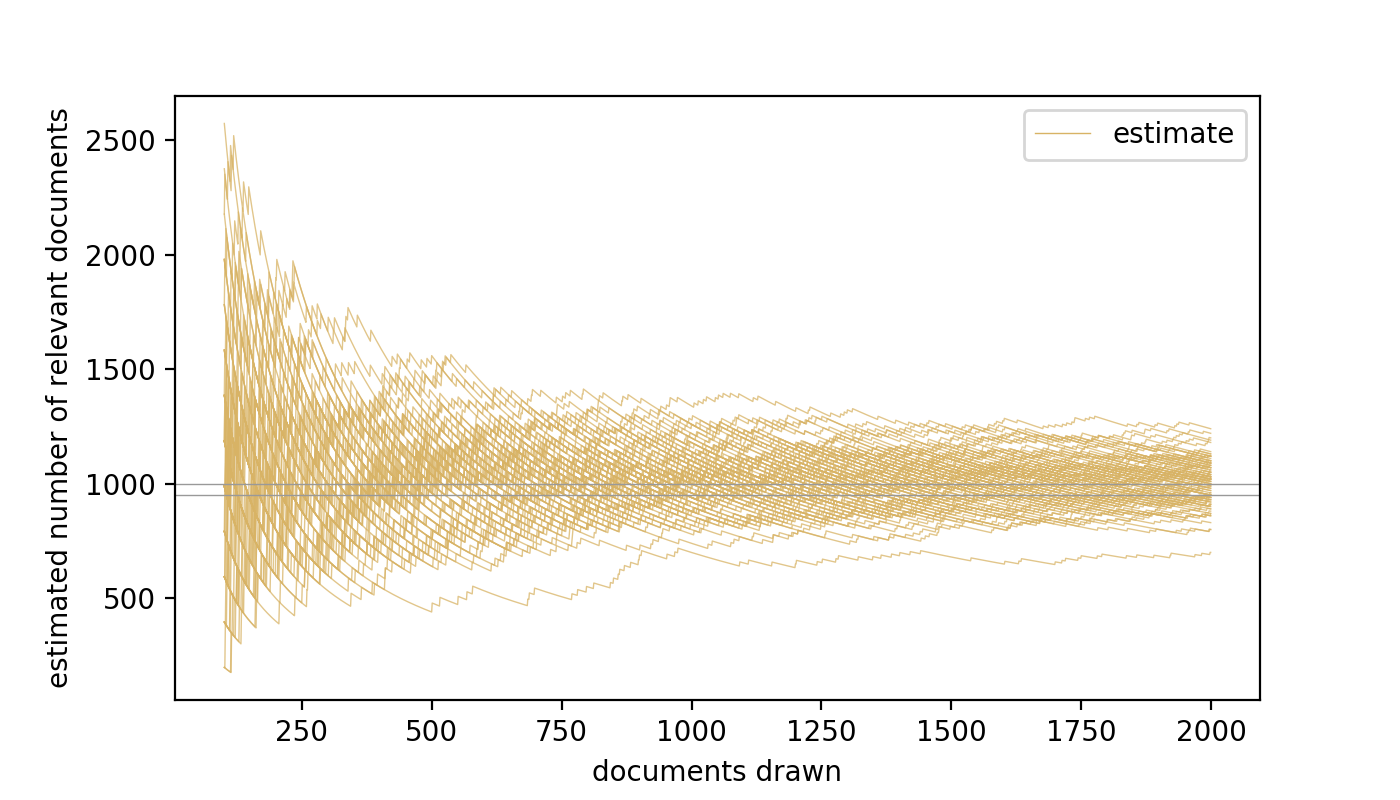
\includegraphics[width=\linewidth]{../images/bir_sampling_noci.png}
	\caption{Uncertainty in estimating the baseline inclusion rate. For 50 random samples of 2,000 documents from 20,000 documents, we show the estimated number of relevant documents, after each document is drawn. The two horizontal grey  lines correspond to the actual number of relevant documents, and to $\frac{100}{0.95}$\% of relevant documents.
		\label{bir-sampling}
	}
\end{figure}

\begin{figure}
	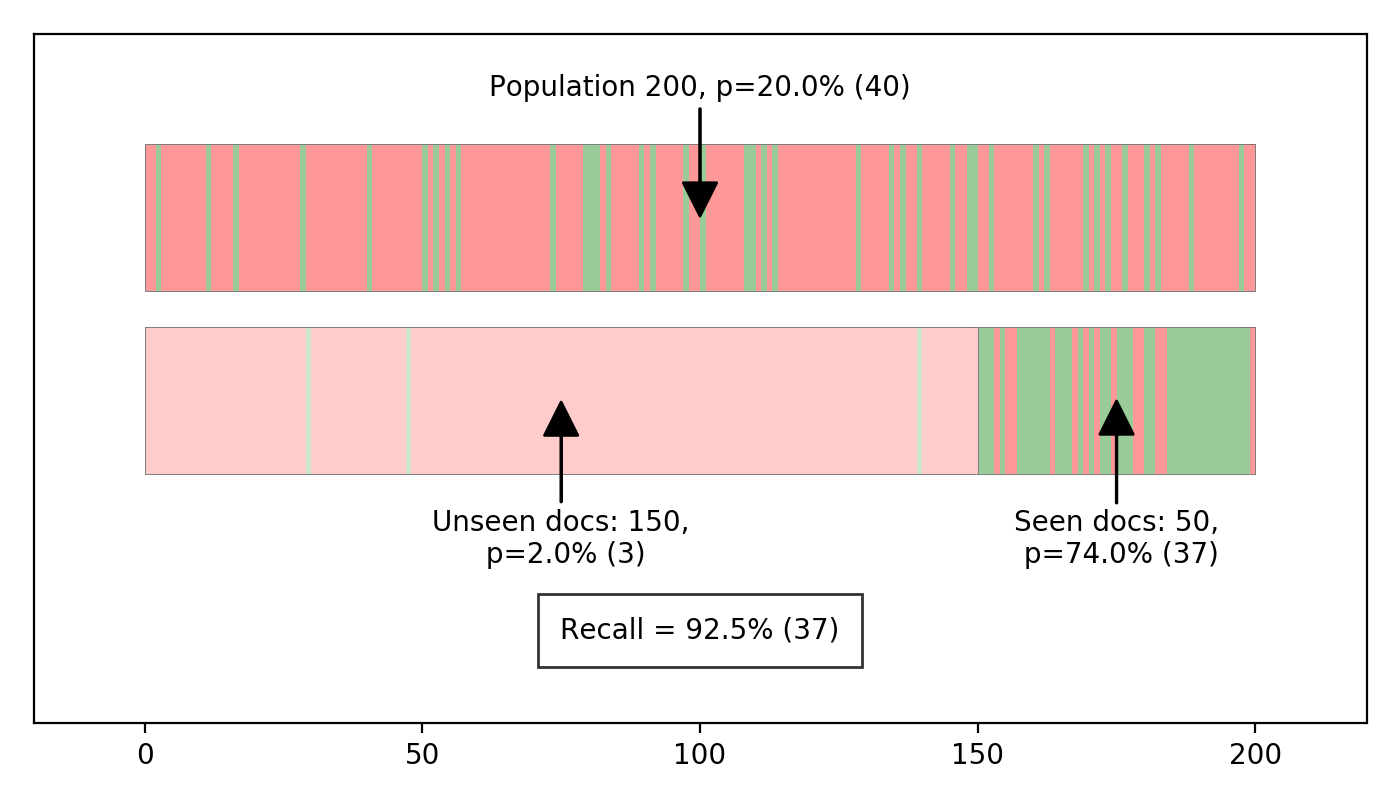
\includegraphics[width=\linewidth]{../images/proportions_1.png}
	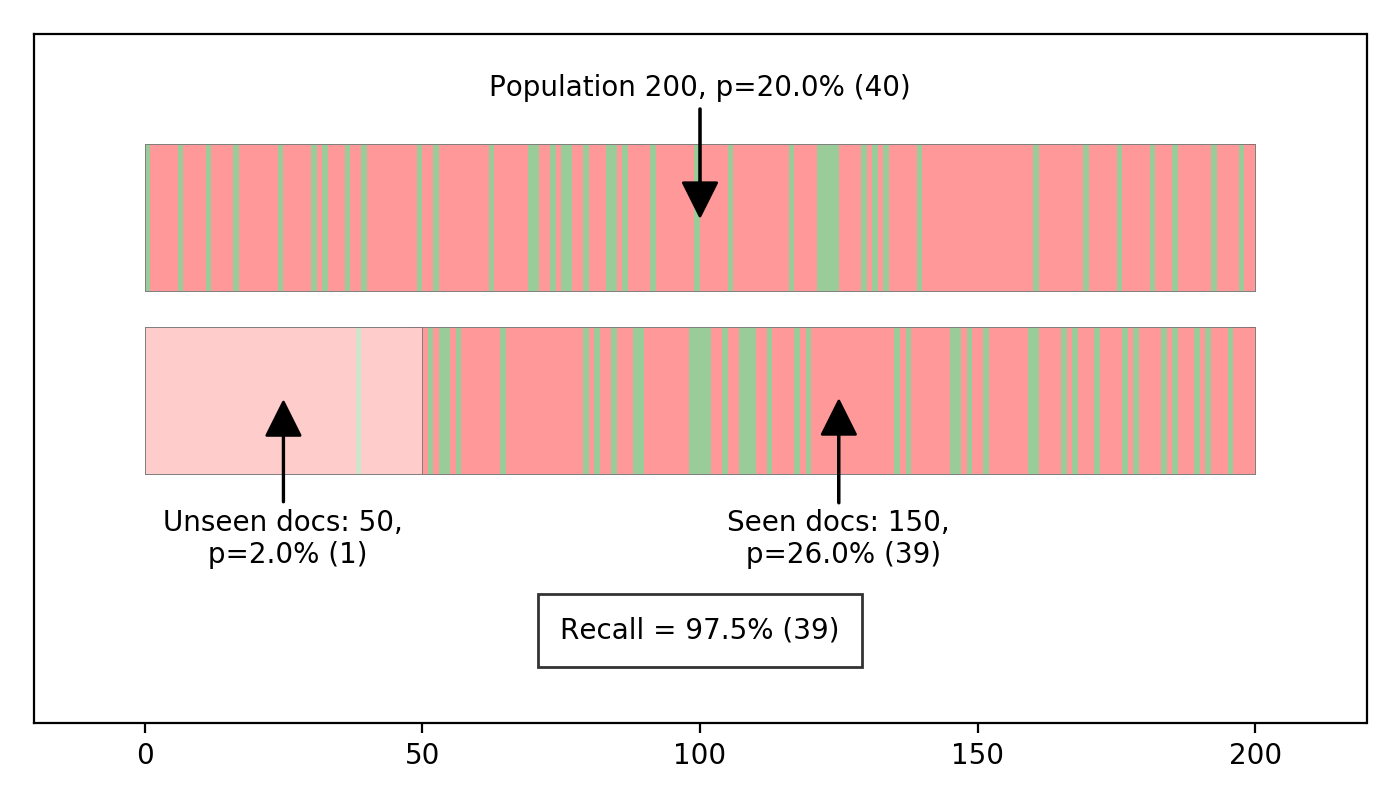
\includegraphics[width=\linewidth]{../images/proportions_2.png}
	\caption{Similar low proportions of relevant documents in unseen documents with different consequences for recall. The top bar shows a random distribution of relevant documents (green) and irrelevant documents (red) at a given proportion of relevance. The bottom bar  shows distributions of relevant and irrelevant documents in hypothetical sets of seen (right) and unseen (left - transparent) documents.}
	\label{unseen-proportions}
\end{figure}


		
\subsubsection*{Heuristic Stopping Criteria}

Some studies give the example of heuristic stopping criteria based on drawing a given number of irrelevant articles in a row \cite{Jonnalagadda2013, Przybya2018}. 
We take this as a proxy for estimating that the proportion of documents remaining in the unseen documents is low. 
We find this a promising intuition, but argue that 1) it ignores uncertainty, as discussed in relation to the previous method; and 2) it misunderstands the significance of a low proportion of relevant documents in estimating the recall.

Figure \ref{unseen-proportions} illustrates this second point. 
We show two scenarios with identical low proportions of relevant documents observed in the unseen documents.
In the top figure, machine learning (ML) has performed well, and 74\% of the seen documents were relevant. 
In the bottom figure,  ML has performed less well, and only 26\% of the seen documents were relevant.
In both cases, only 2\% of unseen documents are relevant, but 2\% of a larger number means more relevant documents are missed.
Recall is not simply a function of the relevance of unseen documents, but also of the number of unseen documents. 
This also means that where ML has performed well (as in the top figure), a low proportion of relevant documents in those not yet checked is indicative of lower recall than where ML has performed less well.
Likewise, where the proportion of relevant documents in the whole corpus is low, a similarly low proportion of relevant documents is likely to be observed, even when true recall is low.



\subsubsection*{Other stopping criteria}

Wallace et al. \cite{Wallace2010a} develop a ``simple, operational stopping criterion'': stopping after half the documents have been screened. Although the criterion worked in their experiment, it is unclear how this could be generalised, and its development depended on knowledge of the true relevance values. 
Jonnalagadda and Petitti \cite{Jonnalagadda2013} note that ``the reviewer can elect to end the process of classifying documents at any point, recognizing that stopping before reviewing all documents involves a trade-off of lower recall for reduced workload'', although clearly the reviewer lacks information about probable recall.
Yu and Menzies \cite{Yu2019} adopt a more complicated stopping criterion which allows the user to target a specific level of recall. However, reviewers are not given the opportunity to specify a confidence level, and for two of the four datasets in which they tested their criteria, the median achieved recall at a stopping criteria targeting 95\% recall was below 95\%. Di Nunzio \cite{DiNunzio2018} also present an innovative stopping criteria, but it does not take into account uncertainty, and produces results \textit{near} a target recall threshold, rather than above it in a reliable proportion of cases. 
These last examples are promising developments, but fail to take into account the needs of live systematic reviews, where the reliability of and ease of communication about recall are paramount.


\subsection*{A Statistical Stopping Criterion for Active Learning}

	\subsubsection*{Random Sampling}
	
	After using machine learning to select which documents are screened by humans as described above, we begin drawing a random sample from the remaining documents (when this happens is described below). 

	We use random sampling to estimate the probability that a target recall $\tau$ has been achieved. Because we are sampling a binary outcome without replacement, we can use the hypergeometric distribution to formulate a statistical test. The hypergeometric distribution tells us the probability of observing $k$ relevant documents in $n$ draws from a finite population of $N$ documents with $K$ relevant documents. 
	
	\begin{equation}
		k \sim Hypergeometric(N, K, n)
	\end{equation}
	
	In our case, we know $k$, $n$ and $N$ after each draw, but $K$ is unknown. We therefore substitute a hypothetical value $\hat{K}$: the minimum number of relevant documents in the sample had the recall target been missed.
	
	Recall $R$ is given by the number of relevant documents that have been seen $\rho_{s}$ over the number of relevant documents in the whole dataset $\rho_{tot}$
	
	\begin{equation}
		R = \frac{\rho_{seen}}{\rho_{tot}}
	\end{equation}
	
	The number of relevant documents in the whole dataset is the sum of $\hat{\rho}$ relevant documents seen before random sampling began and $\tilde{K}$ relevant documents unseen at the start of random sampling. We can therefore express $R$ as
	
	\begin{equation}
		R = \frac{\dot{\rho}}{\hat{\rho} + \tilde{K}},
	\end{equation}
	
	Substituting the target recall $\tau$ for $R$, reorganising and rounding up to the next integer, we can, after each draw, calculate $\hat{K}$, which is the minimum number of relevant documents that could have been remaining when random sampling started, if recall were lower than the target.
	
	\begin{equation}
		\hat{K} = \lceil \frac{\rho}{\tau} - \hat{\rho} \rceil
	\end{equation}
	
	We use the cumulative distribution function of the hypergeometric distribution to estimate the probability $p$ of having observed $k$ or fewer relevant documents in the sample given $\hat{K}$. This function gives us an upper bound on the probability of observing maximally the number of relevant documents in our random sample as we did, if our recall target had not been achieved.
	If this is below our confidence level $1 - \alpha$, we can reject the null hypothesis that the recall target was not achieved.
	
	
	
	
	%%%%%%%%%%%
%	
%	We calculate a hypothetical value $\hat{K}$
%
%	Our aim is to formulate a stopping criterion such that a recall of $\tau$ has been reached with confidence level $\alpha$.
%	To achieve this, we formulate a hypothesis test:
%	We first calculate the number $\hat{n}$ of relevant documents that can maximally remain in the unseen documents to achieve a given recall target. The recall is defined as the ratio of seen relevant documents over all relevant documents
%
%	with the total number of seen relevant documents $\rho$, the number of seen relevant documents at the time we start random sampling $\hat{\rho}$, and the remaining number of relevant documents in the unseen sample at the time random sampling starts $\tilde{n}$.
%	Reorganization of this equation gives
%	\begin{equation}
%		\tilde{n} = \frac{\rho}{\tau} - \hat{\rho}.
%	\end{equation}
%	Because we need to use integers, we get the next largest integer given by the ceiling function $\lceil \cdot \rceil$:
%
%	The null-hypothesis to reject can then be formulated as:
%	\begin{quote}
%	$H_0$: There are $\hat{n}$ or more relevant documents remaining in the set of unseen documents.
%	\end{quote}
%	
%	% notation here follows notation for scipy description of hypergeometric distribution
%	% better use another notation more in line with the literature? -> literature seems to use very different notations
%	
%	In theory, we draw a random sample of $N$ documents, evaluate how many of them are relevant, and denote this number with $k$. We can estimate the probability that we observe $k$ or fewer relevant documents in a random draw of $N$ documents without replacement from a pool of $M$ documents, of which $n$ are relevant using the cumulative distribution function of the hypergeometric distribution.
%This function is defined as the sum over the probability mass function of the hypergeometric distribution $p(x, M, n, N)$:
%	\begin{equation}	
%		 cdf(k, M, n, N) = \sum_{x \leq k} p(x, M, n, N) = \sum_{x \leq k} \frac{\binom{n}{x} \binom{M - n}{N - x}} {\binom{M}{N}},
%		 \label{pfunc}
%	\end{equation}
%	where $\binom{a}{b}$ denote binomial coefficients. In our case, $M$ is the number of unseen documents before we start random sampling.
%	
%	We can reject the null hypothesis if the p-value $p = cdf(k,M,\hat{n},N)$ is smaller than $1 - \alpha$ [references to hypergeometric testing?, needs further argumentation?]. Because we are testing for the lower tail, this implies that we can be confident with a level $\alpha$ that the number of unseen relevant documents is lower than $\hat{n}$.
%	
%	In practice, we can draw random unseen documents repeatedly. After each draw, we calculate the p-value using the number of relevant documents $k$ and the number of randomly sampled documents $N$.
%	We can stop the screening once a p-value $p < 1 - \alpha$ is reached.


	\subsubsection*{Pseudo-random sampling}
	
	In order to decide when to begin a random sample, we employ pseudo-random sampling, where we treat previously screened documents as a random sample. The distribution of relevant documents among previously screened documents is clearly not random, as documents predicted to be relevant are prioritised. It is reasonable to assume, though, that the density of relevant documents is greater among previously screened documents than among remaining unseen documents. This would make the following estimates conservative. 
	
	After reviewing each document, $S$ documents have been screened, and $U$ documents are yet to be seen. We treat $i = 1 \dots S$ of the previously screened documents as a random sample, and calculate $p$, using the method above, for each sample, taking the minimum across all samples $p_{min}$. If $p_{min}$ is less than $1-\frac{\alpha}{2}$, we switch to random sampling. We also calculate $p_{min}$ for the remaining documents as if we had not switched to random sampling and record the recall and work saved when $p_{min} < 1 - \alpha$. We present these in the results below as the psuedo-random sampling criterion.


	\medskip
	
	\begin{figure}
		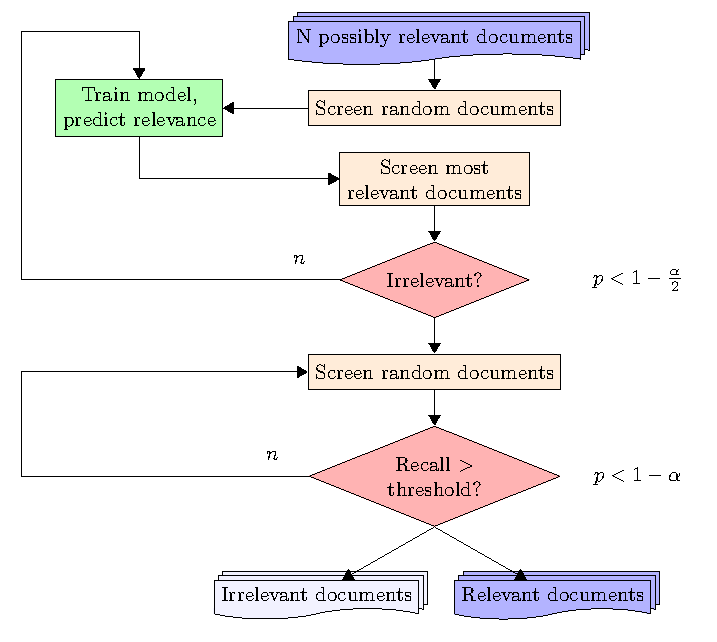
\includegraphics[width=0.5\linewidth]{../images/flow}
		\caption{A workflow for active learning in screening with a statistical stopping criterion}
		\label{flow}
	\end{figure}

	%\subsection*{Analysis}
%	
%	\begin{table}
%		\begin{tabular}{p{0.15\linewidth} p{0.425\linewidth} p{0.425\linewidth}}
%			Parameter & Description & Estimation \\
%			\hline
%			$ P  $ &  Total number of studies & \textit{Observed} \\
%			$ S $ & Number of studies coded by humans & \textit{Observed} \\
%			$ U $ & Number of studies not yet coded by humans & \textit{Observed} ($P - S$) \\
%			$ \alpha $ & Acceptable uncertainty level & \textit{Given} \\
%			$ \tau $ & Target recall threshold & \textit{Given} \\
%			$ k $ & Number of relevant documents drawn & \\
%			$ N $ & Number of randomly drawn documents & \textit{Observed} \\
%			$ M $ & Number of remaining unseen documents before sampling & \\
%			$ n $ & Number of relevant documents in sample & \\
%			$ \hat{n} $ & Minimum number of relevant documents in sample that would mean the recall threshold had been reached  & \\
%		\end{tabular}
%		\caption{Parameters}
%		\label{parameters}
%	\end{table}

	

%
%	
%	Table \ref{parameters} shows the parameters, known, estimated, and given, available during the random sampling process and required to estimate recall. 
%	Expanding on what was stated before, recall - at a given confidence threshold is a function of 1) the upper estimate of the relevance of remaining documents, 2) The estimated relevance of all documents in the dataset, 3) The proportion of documents not yet seen. 
%	
%	Figure \ref{sample-recall} shows the minimum estimated recall for a set of confidence intervals, along with the actual recall (in grey) for a case where 800 out of 2,000 documents have been reviewed, 2\% of remaining documents are relevant, and 20\% of all documents are relevant. 
%	We see that after 95\% recall has actually been achieved, but before 100\% of documents have been been seen, we can be confident at each of the given confidence levels that 95\% of relevant documents have been identified. 
%	All estimates of recall only reach 100\% after all documents have been seen, as it is not possible to exclude the possibility, at any given confidence level, that the proportion of relevant documents is greater than 0 \todo{Actually maybe this is possible if we work with whole numbers? How does that change things?}. 
%	Figure \ref{sample-recall-variation} shows the various trajectories of a 95\% minimum recall (blue) and actual recall (grey) given the same paramaters for 200 random samples.
%
%	That the blue lines consistently meet a 95\% threshold to the right of the grey lines indicates that reviewers have to see more than 95\% of relevant documents in order to be confident that they have achieved their threshold. 
%	We call the number of documents it is necessary to review to establish with confidence that reviewers have achieved 95\% recall after they have already achieved 95\% recall the \textit{additional burden}. 
%	
%	In figure \ref{additional-burden}, we investigate how the total number of documents and the proportion of relevant documents affect the additional burden \todo{Use the number of documents seen instead of p?}. We demonstrate the additional burden decreases \todo{how? Non-linearly?} with increasing total numbers of documents. With decreasing relevance of the remaining documents (holding the recall constant at 95\%, this means that fewer documents remain unseen), the additional burden increases. This implies that where the machine learning has more successfully identified documents and reduced burden, the additional burden required to establish the level of recall is higher. This is because the proportion of documents not seen is greater, so uncertainty around the relevance of that proportion has a greater impact on the estimation of recall.
%
%	When to move to random sampling remains an open question. Our current approach is to use the predicted relevance of the machine learning model as a guide. We calculate the [minimum/maximum] estimated recall based on observing the predicted relevance level in [x] random documents. If the estimated recall would be below the threshold, then we begin drawing random documents.
%
%	The stopping criteria explained here is 
	
	\subsection*{Evaluation}
	
	We evaluate each of the criteria discussed on real world test data, operationalising the heuristic stopping criterion with 50, 100, and 200 consecutive irrelevant records. We run 100 iterations on each dataset and record the following measures.
	\begin{itemize}
		\item \textbf{Actual Recall}: The recall when the stopping criterion was met
		\item \textbf{WS-SC}: Work saved when the stopping criterion was met \footnote{We do not use work saved over sampling, it is not axiomatic that seeing 95\% of a random sample would achieve 95\% recall}
		\item \textbf{Additional Burden}: the work saved when the criterion was triggered subtracted from the work saved when the recall target was actually achieved.

	\end{itemize}
	For simplicity, we use a basic SVM model \cite{Cortes95, Pedregosa2011}, with 1-2 word n-grams taken from the document abstracts used as input data. We start with random samples of 200 documents. Subsequently, we ``screen'', that is, we reveal the labels of batches of the 20 documents with the highest predicted relevance scores, retraining the model after each batch. Each criterion is evaluated after each document is ``screened''.
	 For our criteria, we set the target recall value to 95\% and the confidence level to 95\%.
	
	
	%\subsubsection*{Evaluation Data}
	\begin{table}
		\begin{tabular}{lllrrr}
\toprule
{} &                  dataset & data\_source &     N &  r\_docs &    p \\
\midrule
0  &      UrinaryIncontinence &       cohen &   284 &      68 & 0.24 \\
1  &           Antihistamines &       cohen &   287 &      90 & 0.31 \\
2  &                Estrogens &       cohen &   349 &      79 & 0.23 \\
3  &                   NSAIDS &       cohen &   358 &      83 & 0.23 \\
4  &        OralHypoglycemics &       cohen &   475 &     135 & 0.28 \\
5  &                 Triptans &       cohen &   594 &     205 & 0.35 \\
6  &                     ADHD &       cohen &   803 &      83 & 0.10 \\
7  &   AtypicalAntipsychotics &       cohen &  1030 &     333 & 0.32 \\
8  &   CalciumChannelBlockers &       cohen &  1103 &     257 & 0.23 \\
9  &     ProtonPumpInhibitors &       cohen &  1210 &     227 & 0.19 \\
10 &  SkeletalMuscleRelaxants &       cohen &  1348 &      30 & 0.02 \\
11 &                     COPD &     copd\_pb &  1443 &     179 & 0.12 \\
12 &               Kitchenham &    fastread &  1700 &      45 & 0.03 \\
13 &                   Opiods &       cohen &  1769 &      43 & 0.02 \\
14 &             BetaBlockers &       cohen &  1872 &     270 & 0.14 \\
15 &            ACEInhibitors &       cohen &  2234 &     168 & 0.08 \\
16 &                  Statins &       cohen &  2743 &     152 & 0.06 \\
17 &               ProtonBeam &     copd\_pb &  4108 &     240 & 0.06 \\
18 &               Radjenovic &    fastread &  5999 &      47 & 0.01 \\
19 &                   Wahono &    fastread &  7002 &      62 & 0.01 \\
20 &                     Hall &    fastread &  8911 &     104 & 0.01 \\
\bottomrule
\end{tabular}

		\caption{Dataset properties}
		\label{tab:data}
	\end{table}
	
	The systematic review datasets used for testing are described in table \ref{tab:data}. We use the seminal collection of systematic reviews used to develop machine learning applications for document screening by Aaron Cohen and co-authors in 2006 \cite{Cohen2006}, along with the widely used Proton Beam \cite{Terasawa2009} and COPD \cite{Castaldi2009} datasets, and computer science datasets used to test FASTREAD \cite{Yu2019}. Testing on datasets with different properties and from different domains is key to establishing criteria appropriate for general use. Choosing as broad as possible data also prevents us from being able to ``tune'' our machine learning approach in ways that may work well for specific datasets but not generalise well. Work savings, even maximum work savings are therefore below the state of the art recorded for each of these datasets. In this way we can show how well the criteria perform even when the model performs badly.
	
	%As a last step, we explain the factors that increase or decrease the performance of our criteria, using a simple regression model.
	
	\section*{Results}
	
	Figure \ref{recall-wss} shows the actual recall and work savings achieved when each stopping criterion has been satisfied. 
	For comparison, we also include the results that would have been achieved with \textit{a priori} knowledge of the data, that is, the work saved when the 95\% recall target was actually reached. In a live systematic review, reviewers would never know when this had been reached, but these are the work savings most often reported in machine learning for systematic review screening studies.
		
	The baseline sampling criterion (Figure \ref{fig:bir}) misses the 95\% recall target in 39.67\% of cases, while the most common work saving is 0\%. This is in line with our expectations that, due to random sampling error, the expected number of documents will often be over-estimated or under-estimated, resulting in zero work savings or poor recall.

    \begin{figure*}
	\centering
	\begin{subfigure}[b]{0.475\textwidth}
		\centering
		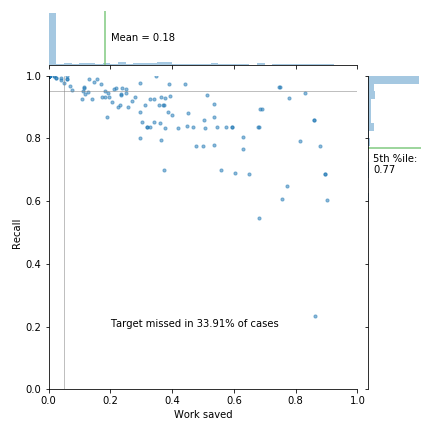
\includegraphics[width=\textwidth]{../images/jointplot_bir}
		\caption[Network2]%Example-Image
		{{\small Baseline Sampling}}    
		\label{fig:bir}
	\end{subfigure}
	\hfill
	\begin{subfigure}[b]{0.475\textwidth}  
		\centering 
		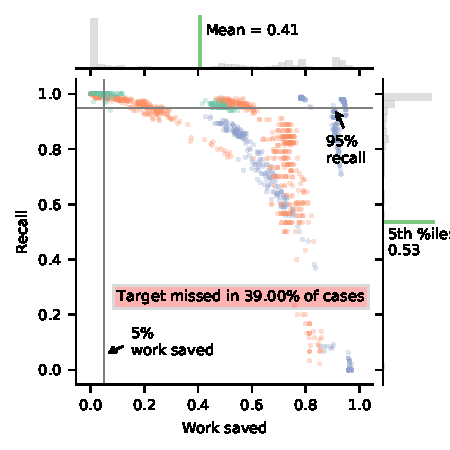
\includegraphics[width=\textwidth]{../images/jointplot_ih_50}
		\caption[]%
		{{\small 50 consecutive irrelevant results}}    
		\label{fig:ih_50}
	\end{subfigure}
	\vskip\baselineskip
	\begin{subfigure}[b]{0.475\textwidth}   
		\centering 
		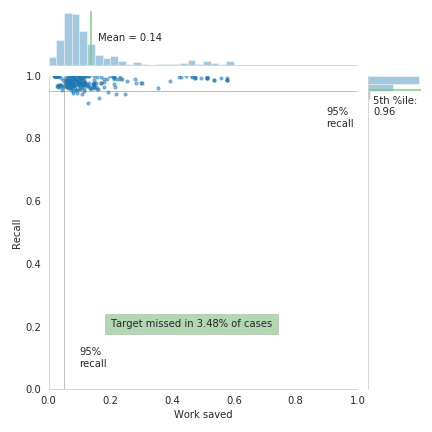
\includegraphics[width=\textwidth]{../images/jointplot_hyper}
		\caption[]%
		{{\small Hypergeometric sampling \\}}    
		\label{fig:hyper}
	\end{subfigure}
	\hfill
	\begin{subfigure}[b]{0.475\textwidth}   
		\centering 
		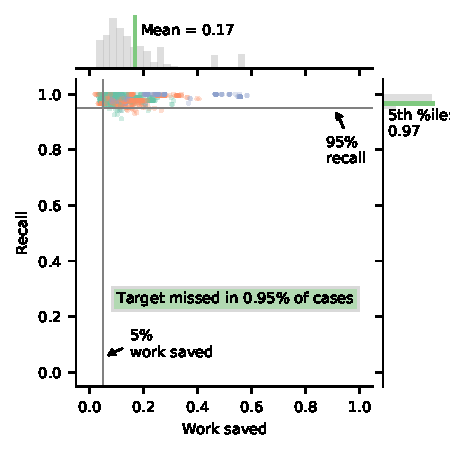
\includegraphics[width=\textwidth]{../images/jointplot_nrs}
		\caption[]%
		{{\footnotesize Pseudorandom hypergeometric sampling}}    
		\label{fig:nrs}
	\end{subfigure}
	\vskip\baselineskip
	\begin{subfigure}[b]{0.475\textwidth}   
		\centering 
		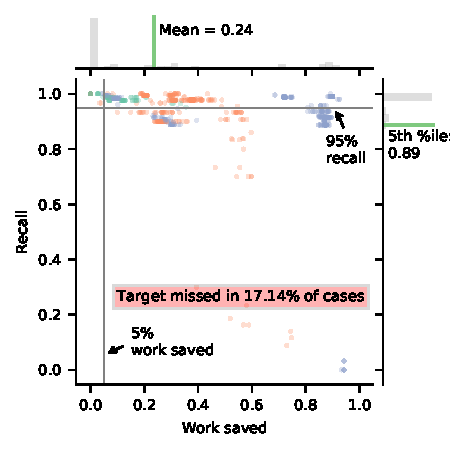
\includegraphics[width=\textwidth]{../images/jointplot_ih_200}
		\caption[]%
		{{\small 200 consecutive irrelevant results \\}}    
		\label{fig:ih_200}
	\end{subfigure}
	\hfill
	\begin{subfigure}[b]{0.475\textwidth}   
		\centering 
		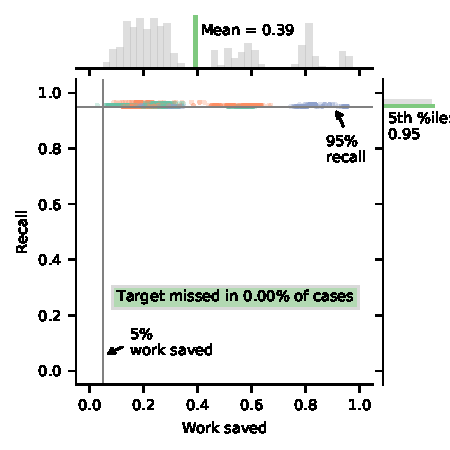
\includegraphics[width=\textwidth]{../images/jointplot_pf.pdf}
		\caption[]%
		{{\footnotesize \textit{a priori} knowledge}}   
		\label{fig:pf}
	\end{subfigure}

	\caption{\small Distribution of recall and work saved after each stopping criterion. Green dots show results for datasets with less than 1,000 documents, orange dots show datasets with 1,000 - 2,000 documents, and blue dots show datasets with more than 2,000 documents.} 
	\label{recall-wss}
\end{figure*}

\begin{figure*}
	\centering
	\begin{subfigure}[b]{0.475\textwidth}
		\centering
		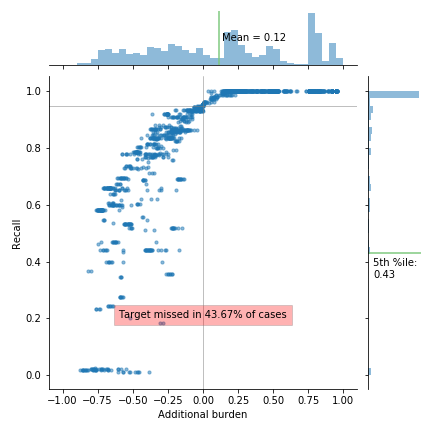
\includegraphics[width=\textwidth]{../images/jointplot_burden_bir}
		\caption[Network2]%Example-Image
		{{\small Baseline Sampling}}    
		\label{fig:bir_ab}
	\end{subfigure}
	\hfill
	\begin{subfigure}[b]{0.475\textwidth}  
		\centering 
		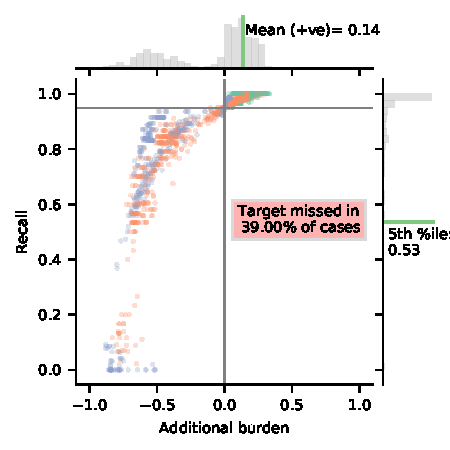
\includegraphics[width=\textwidth]{../images/jointplot_burden_ih_50}
		\caption[]%
		{{\small 50 consecutive irrelevant results}}    
		\label{fig:ih_50_ab}
	\end{subfigure}
	\vskip\baselineskip
	\begin{subfigure}[b]{0.475\textwidth}   
		\centering 
		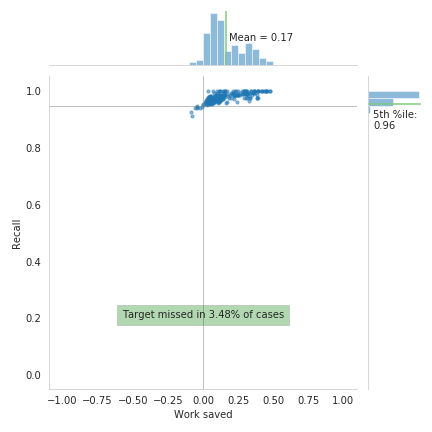
\includegraphics[width=\textwidth]{../images/jointplot_burden_hyper}
		\caption[]%
		{{\small Hypergeometric sampling \\}}    
		\label{fig:hyper_ab}
	\end{subfigure}
	\hfill
	\begin{subfigure}[b]{0.475\textwidth}   
		\centering 
		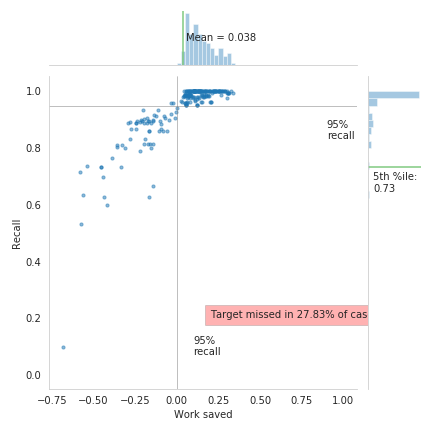
\includegraphics[width=\textwidth]{../images/jointplot_burden_ih_100}
		\caption[]%
		{{\small 100 consecutive irrelevant results }}    
		\label{fig:ih_200_ab}		

	\end{subfigure}
	\vskip\baselineskip
	\begin{subfigure}[b]{0.475\textwidth}   
		\centering 
		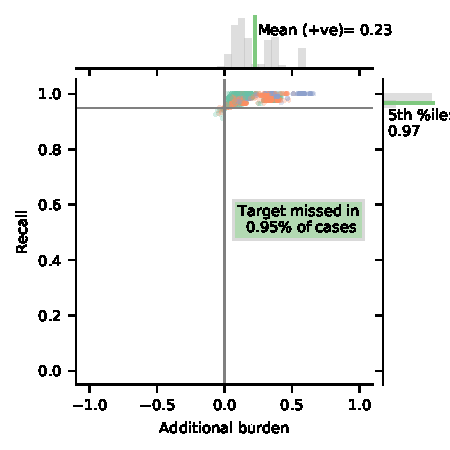
\includegraphics[width=\textwidth]{../images/jointplot_burden_nrs.pdf}
		\caption[]%
		{{\footnotesize Pseudorandom hypergeometric sampling}}    
		\label{fig:nrs_ab}
	\end{subfigure}
	\hfill
	\begin{subfigure}[b]{0.475\textwidth}   
		\centering 
		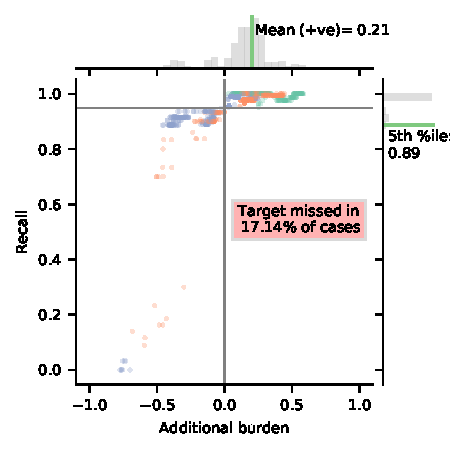
\includegraphics[width=\textwidth]{../images/jointplot_burden_ih_200.pdf}
		\caption[]%
		{{\footnotesize 200 consecutive irrelevant results }}    
		\label{fig:ih_100_ab}
	\end{subfigure}
	
	\caption{\small Distribution of recall and additional burden after each stopping criterion. Additional burden is the work saved when the criterion was triggered minus the work saved when the target was reached. Coloring of data points as in Fig. \ref{recall-wss}.}
	\label{recall-burden}
\end{figure*}


	The Heuristic stopping criteria, both for 50 consecutive irrelevant results (Figure \ref{fig:ih_50} - IH50), and for 200 irrelevant results (Figure \ref{fig:ih_200}) also perform unreliably. Although the mean work saved for IH50 is 41\%, the target is missed in 39\% of cases. The cases below the horizontal grey line indicate instances where work has been saved at the expense of achieving the recall target.
	
	Both the random sampling and the pseudorandom sampling criteria achieve the target threshold of 95\% in more than 95\% of cases. In fact, the pseudorandom sampling criterion  outperforms the random sampling criterion with respect to both recall and work savings. In theory, the pseudorandom sampling criteria is conservative if the assumption holds that documents chosen by machine learning are not less likely to be relevant than those chosen at random. Based on our experiments, this assumption seems reasonable, and accounts for the higher recall. Because the pseudorandom sampling criterion can flexibly choose its sample, whereas the random criterion has to wait for a random sample to be triggered, the criterion is also triggered earlier, as it can make use of more data. This accounts for the higher work savings.
	
	\begin{figure}
		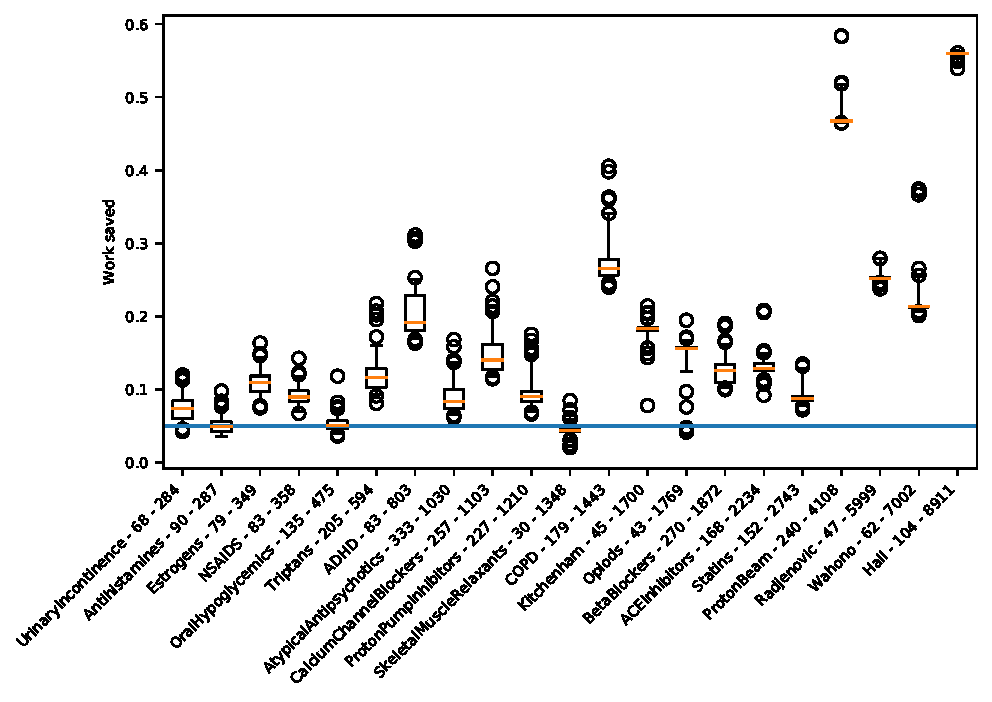
\includegraphics[width=0.9\linewidth]{../images/wss_nrs}
		\caption{Work saved for the pseudorandom sampling method in each dataset. Labels show the number of relevant documents and the total number of documents. The datasets are presented in order of the number of documents. The whiskers represent the 5th and 95th percentiles.}
		\label{wss}
	\end{figure}
	
 	\begin{figure*}
		\centering
		\begin{subfigure}[b]{0.475\textwidth}
			\centering
			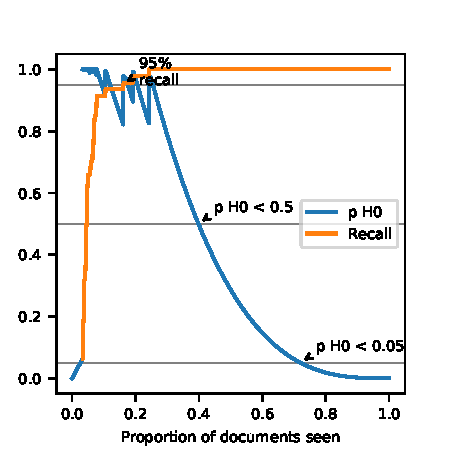
\includegraphics[width=\textwidth]{../images/h0_paths_Radjenovic.pdf}
			\caption[Network2]%Example-Image
			{{\small Radjenovic}}    
			\label{fig:Radjenovic}
		\end{subfigure}
		\hfill
		\begin{subfigure}[b]{0.475\textwidth}  
			\centering 
			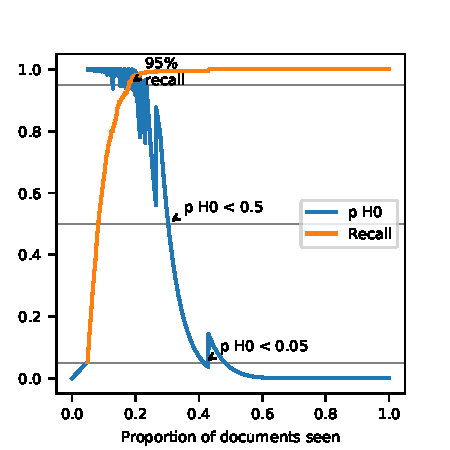
\includegraphics[width=\textwidth]{../images/h0_paths_ProtonBeam.pdf}
			\caption[]%
			{{\small ProtonBeam}}    
			\label{fig:ProtonBeam}
		\end{subfigure}
	\vskip\baselineskip
		\begin{subfigure}[b]{0.475\textwidth}
			\centering
			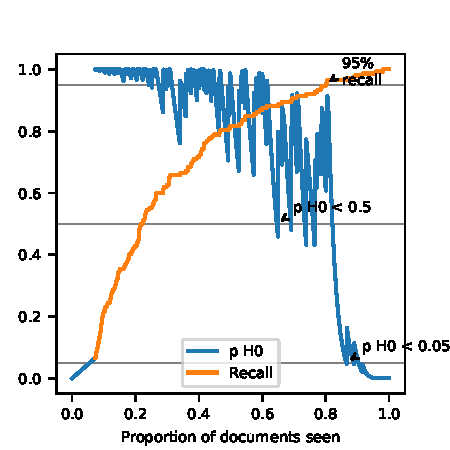
\includegraphics[width=\textwidth]{../images/h0_paths_Statins.pdf}
			\caption[Network2]%Example-Image
			{{\small Statins}}    
			\label{fig:Statins}
		\end{subfigure}
		\hfill
		\begin{subfigure}[b]{0.475\textwidth}  
			\centering 
			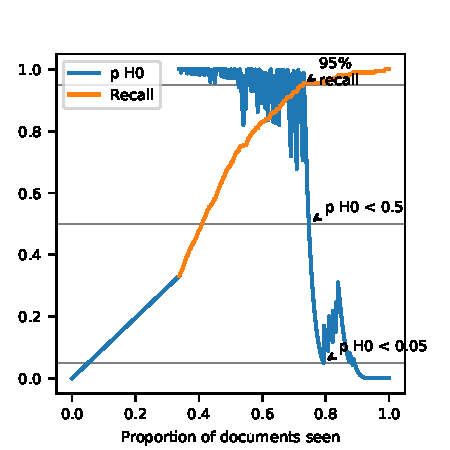
\includegraphics[width=\textwidth]{../images/h0_paths_Triptans.pdf}
			\caption[]%
			{{\small Triptans}}    
			\label{fig:Triptans}
		\end{subfigure}
	
		\caption{\small The path of recall (yellow) and the p-value of H0 for four different datasets} 
		\label{H0paths}
	\end{figure*}
	
	In figure \ref{recall-burden} we rescale the x axis, calling it additional burden, which is simply the work saved when the criterion is triggered subtracted from the work saved when the recall target was actually achieved. This measure indicates whether the stopping criterion was triggered too early (positive values), or too late (negative values). The figure directly highlights the tradeoffs involved in deciding when to stop screening. 
	
	To help explain the different work savings that were observed in our experiments, we show the distribution of work savings from our pseudorandom criterion for each dataset in figure \ref{wss}. In general, higher work savings are possible when the total number of documents is larger. However, in datasets with a low proportion of relevant documents, many documents need to be screened to achieve a high confidence that there are only few relevant documents remaining in the unseen ones. Therefore, smaller work savings are possible. 
	
	Figure \ref{H0paths} shows the recall and the probability of the null hypothesis for the best performing iteration of four datasets. Although the 95\% recall target is achieved very quickly in the Radjenovic dataset, the null hypothesis cannot be excluded until much later. This is because the dataset has only 47 relevant documents out of a population of 5,999. After the 95\% recall target was achieved, 45 out of 47 relevant documents had been seen and 5,029 documents remained. The null hypothesis was therefore that 3 or more of these 5,029 documents were relevant, which requires a lot of evidence to disprove. The burden of proof was smaller in the case of the Proton Beam dataset: at the point that the 95\% recall threshold was reached, the null hypothesis to disprove was that 13 out of 3,369 remaining documents were relevant. 
	
	The Statins and Triptans datasets show how the criterion performs when the machine learning model has performed poorly in predicting relevant results. In each case, 95\% recall is achieved with close to 20\% of documents remaining. With fewer documents remaining, it takes less screening to rule out the possibility that the number of relevant documents left is incompatible with the achievement of the recall target.
	
	\section*{Discussion}
	
	Our results show that it is possible to use machine learning to achieve a given level of recall with a given level of confidence. The tradeoff for achieving recall reliably is that the work saving achieved is less than the maximum possible work saving. However, for large datasets with a significant proportion of relevant documents, the additional effort required to satisfy the criterion will be small. This makes the approach well suited to broad topics with lots of literature. In other words, it is precisely where machine learning will be most useful that the additional effort will be small.
	
	Different use cases for machine learning enhanced screening may also carry different requirements for recall, or different tolerances for uncertainty. These can be flexibly accommodated within our stopping criterion. Importantly, the ability to make probabilistic statements about the chance of achieving a given recall target makes it possible to clearly communicate the implications of using machine learning enhanced screening to readers and reviewers who are not machine learning specialists. This is extremely important in live systematic reviews. 
	
	Our criterion has the further advantage that it is independent of the choice or performance of the machine learning model. If a model performs badly at discerning relevant from irrelevant results, the only consequence will be that the work saved will be low. With other criteria this may result in poor recall. 
	When using machine learning for screening, poor recall can result in biased results, while low work savings represent no loss to the reviewer as compared to not using machine learning.
	
	So far, systematic review standards have no way of accommodating screening with machine learning. 
	We hope that the reliability and clarity of reporting offered by our stopping criterion make them suitable for incorporation into standards, so that machine learning for systematic review screening can fulfil its promise of reducing workload and making more ambitious reviews tractable.
	
	\section*{Conclusion}
	
	This paper demonstrates the unsuitability of existing stopping criteria for machine learning approaches to document screening, and proposes a simple method that delivers reliable recall, independent of machine learning approach or model performance. Our robust statistical stopping criteria allow users to easily communicate the implications of their use of machine learning, making machine learning enhanced screening ready for live reviews.
	
	
\begin{backmatter}
	
	\section*{Competing interests}
	The authors declare that they have no competing interests.
	
	\section*{Author's contributions}
	MC designed the research and conducted the experiments. FMH contributed to the development of the statistical basis for the stopping criterion. Both authors wrote and edited the manuscript.
	
	\section*{Acknowledgements}
	Max Callaghan is supported by a PhD scholarship from the Heinrich Böll Foundation
		
	\bibliography{mendeley}
	\bibliographystyle{vancouver}
	
\end{backmatter}
\end{document}